\documentclass{article}
\usepackage{fancyhdr}
\usepackage{caption}
\usepackage{tikz}
\pagestyle{fancy}
\lhead{Modo ejemplo}
\rhead{Proyecto II IC6400}
\begin{document}
\section*{Resultados del modo de ejemplo}
\subsection*{I. Descripción del problema}
Se tienen 6 llaves diferentes (A, B, C, D, E y F), cada una de las cuales tiene una probabilidad diferente. A continuaci\'on se muestran dos \'arboles de b\'usqueda binarios. El primero corresponde con el \'arbol binario \'optimo generado por el algoritmo de programaci\'on din\'amica. El segundo es el resultado del algoritmo greedy.
\begin{figure}[ht]
\centering
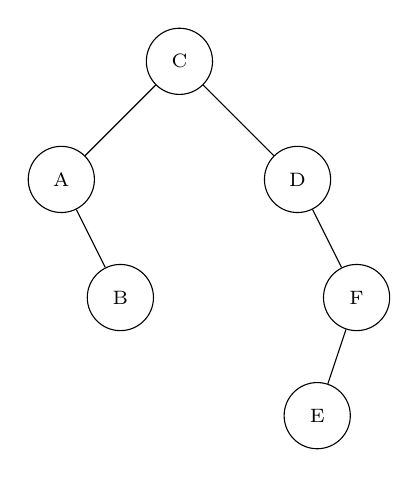
\begin{tikzpicture}[
every node/.style = {minimum width = 3em, draw, circle},
level/.style={sibling distance={3cm/max(1,#1)}}
]
\scriptsize
\node {C}
child {
node {A}
child[missing]
child{
node {B}
}
}
child {node {D}
child[missing]
child{
node {F}
child{
node {E}
}
child[missing]
}
};
\end{tikzpicture}
\caption{\'Arbol generado por el algoritmo de programación din\'mica}
\label{pd}
\end{figure}
\begin{figure}[ht]
\centering
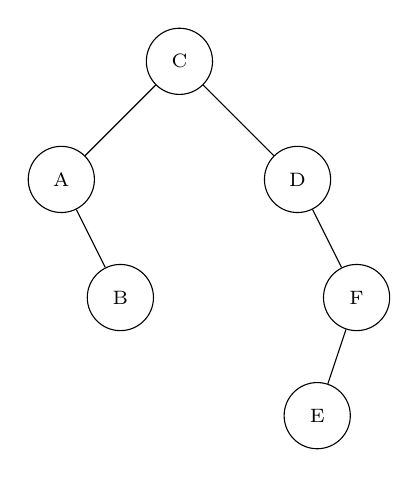
\begin{tikzpicture}[
every node/.style = {minimum width = 3em, draw, circle},
level/.style={sibling distance={3cm/max(1,#1)}}
]
\scriptsize
\node {C}
child {
node {A}
child[missing]
child{
node {B}
}
}
child {node {D}
child[missing]
child{
node {F}
child{
node {E}
}
child[missing]
}
};
\end{tikzpicture}
\caption{\'Arbol generado por el algoritmo greedy}
\label{greedy}
\end{figure}
\end{document}
